%%
%% This is file `main.tex' based on `sample-sigconf.tex' (q.v. for spurce of that,
%%
%% IMPORTANT NOTICE:
%% 
%% For the copyright see the original source file `sample-sigconf.tex'
%% in the `Sample' folder.
%%
%% For distribution of the original source see the terms
%% for copying and modification in the file samples.dtx.
%% 
%% This generated file may be distributed as long as the
%% original source files, as listed above, are part of the
%% same distribution. (The sources need not necessarily be
%% in the same archive or directory.)
%%
%% Commands for TeXCount
%TC:macro \cite [option:text,text]
%TC:macro \citep [option:text,text]
%TC:macro \citet [option:text,text]
%TC:envir table 0 1
%TC:envir table* 0 1
%TC:envir tabular [ignore] word
%TC:envir displaymath 0 word
%TC:envir math 0 word
%TC:envir comment 0 0
%%
%%
%% The first command in your LaTeX source must be the \documentclass command.

%% NOTE that a single column version is required for 
%% submission and peer review. This can be done by changing
%% the \doucmentclass[...]{acmart} in this template to 
%%\documentclass[manuscript,review,anonymous]{acmart}
%% This version is used for drafting and final submission
\documentclass[sigconf]{acmart}


%% 
%% To ensure 100% compatibility, please check the white list of
%% approved LaTeX packages to be used with the Master Article Template at
%% https://www.acm.org/publications/taps/whitelist-of-latex-packages 
%% before creating your document. The white list page provides 
%% information on how to submit additional LaTeX packages for 
%% review and adoption.
%% Fonts used in the template cannot be substituted; margin 
%% adjustments are not allowed.

%%
%% \BibTeX command to typeset BibTeX logo in the docs
\AtBeginDocument{%
  \providecommand\BibTeX{{%
    \normalfont B\kern-0.5em{\scshape i\kern-0.25em b}\kern-0.8em\TeX}}}

%% Rights management information.  This information is sent to you
%% when you complete the rights form.  These commands have SAMPLE
%% values in them; it is your responsibility as an author to replace
%% the commands and values with those provided to you when you
%% complete the rights form.
\setcopyright{acmlicensed}
\copyrightyear{2024}
\acmYear{2024}
\acmDOI{not-applicable}

%% These commands are for a PROCEEDINGS abstract or paper.
\acmConference[TAU]{Workshop in Implementation of Cryptographic Attacks}{2024}{Tel Aviv, IL}
%
%  Uncomment \acmBooktitle if th title of the proceedings is different
%  from ``Proceedings of ...''!
%
%\acmBooktitle{Woodstock '18: ACM Symposium on Neural Gaze Detection,
%  June 03--05, 2018, Woodstock, NY} 
\acmISBN{978-1-4503-XXXX-X/18/06}


%%
%% Submission ID.
%% Use this when submitting an article to a sponsored event. You'll
%% receive a unique submission ID from the organizers
%% of the event, and this ID should be used as the parameter to this command.
%%\acmSubmissionID{123-A56-BU3}

%%
%% For managing citations, it is recommended to use bibliography
%% files in BibTeX format.
%%
%% You can then either use BibTeX with the ACM-Reference-Format style,
%% or BibLaTeX with the acmnumeric or acmauthoryear sytles, that include
%% support for advanced citation of software artefact from the
%% biblatex-software package, also separately available on CTAN.
%%
%% Look at the sample-*-biblatex.tex files for templates showcasing
%% the biblatex styles.
%%

%%
%% The majority of ACM publications use numbered citations and
%% references.  The command \citestyle{authoryear} switches to the
%% "author year" style.
%%
%% If you are preparing content for an event
%% sponsored by ACM SIGGRAPH, you must use the "author year" style of
%% citations and references.
%% Uncommenting
%% the next command will enable that style.
%%\citestyle{acmauthoryear}

%%
%% end of the preamble, start of the body of the document source.

%% % Location of your graphics files for figures, here a sub-folder to the main project folder
\graphicspath{{./images/}} 


\begin{document}

%%
%% The "title" command has an optional parameter,
%% allowing the author to define a "short title" to be used in page headers.
\title{EyalTheSinger: An Extensible Password Brute-Forcing Program}

%%
%% The "author" command and its associated commands are used to define
%% the authors and their affiliations.
%% Of note is the shared affiliation of the first two authors, and the
%% "authornote" and "authornotemark" commands
%% used to denote shared contribution to the research.
\author{Gal Chapman}
\affiliation{%
  \institution{Tel Aviv University}
  \city{Tel Aviv}
  \country{Israel}}
\email{galchapman@gmail.com}

\author{Maya Ben Shalom}
\affiliation{%
  \institution{Tel Aviv University}
  \city{Tel Aviv}
  \country{Israel}}
\email{maya86420@gmail.com}

\author{Eliav Huppert}
\affiliation{%
  \institution{Tel Aviv University}
  \city{Tel Aviv}
  \country{Israel}}
\email{eliavhuppert@mail.tau.ac.il}

\author{Noam Zaks}
\affiliation{%
  \institution{Tel Aviv University}
  \city{Tel Aviv}
  \country{Israel}}
\email{noam@noamzaks.com}

%%
%% By default, the full list of authors will be used in the page
%% headers. Often, this list is too long, and will overlap
%% other information printed in the page headers. This command allows
%% the author to define a more concise list
%% of authors' names for this purpose.
% \renewcommand{\shortauthors}{Trovato and Tobin, et al.}

%%
%% The abstract is a short summary of the work to be presented in the
%% article.
\begin{abstract}
    WPA2 has two major flaws: 1. It has to be used by humans, and 2. it is possible to iterate over passwords offline. More specifically, Wi-Fi passwords are chosen by people, and people are not very good when it comes to password selection. Since given an initial connection to a Wi-Fi network, there is a straightforward formula to calculate the client's Message Integrity Code (MIC) from the passphrase, it is possible to perform a dictionary attack and a brute-force attack on a Wi-Fi password, offline.

    In this project we take advantage of these weaknesses, and design a tool from scratch that implements such an attack. We sniff and analyze connections, extract the 4-way handshake packets, and use the information to perform dictionary and brute force attacks, using our own implementations of all cryptographic functions. Additionally, we create a CTF challenge that aims to guide a participant through creating such a tool on their own, and emphasizes the importance of strong password choices.

\end{abstract}

%%
%% The code below is generated by the tool at: http://dl.acm.org/ccs.cfm
%% Please copy and paste the code instead of the example below.
%%
% \begin{CCSXML}
% <ccs2012>
%  <concept>
%   <concept_id>00000000.0000000.0000000</concept_id>
%   <concept_desc>Do Not Use This Code, Generate the Correct Terms for Your Paper</concept_desc>
%   <concept_significance>500</concept_significance>
%  </concept>
%  <concept>
%   <concept_id>00000000.00000000.00000000</concept_id>
%   <concept_desc>Do Not Use This Code, Generate the Correct Terms for Your Paper</concept_desc>
%   <concept_significance>300</concept_significance>
%  </concept>
%  <concept>
%   <concept_id>00000000.00000000.00000000</concept_id>
%   <concept_desc>Do Not Use This Code, Generate the Correct Terms for Your Paper</concept_desc>
%   <concept_significance>100</concept_significance>
%  </concept>
%  <concept>
%   <concept_id>00000000.00000000.00000000</concept_id>
%   <concept_desc>Do Not Use This Code, Generate the Correct Terms for Your Paper</concept_desc>
%   <concept_significance>100</concept_significance>
%  </concept>
% </ccs2012>
% \end{CCSXML}

% \ccsdesc[500]{Do Not Use This Code~Generate the Correct Terms for Your Paper}
% \ccsdesc[300]{Do Not Use This Code~Generate the Correct Terms for Your Paper}
% \ccsdesc{Do Not Use This Code~Generate the Correct Terms for Your Paper}
% \ccsdesc[100]{Do Not Use This Code~Generate the Correct Terms for Your Paper}

%%
%% Keywords. The author(s) should pick words that accurately describe
%% the work being presented. Separate the keywords with commas.
% \keywords{Do, Not, Us, This, Code, Put, the, Correct, Terms, for,
  % Your, Paper}

%% The following are not a requirement, delete if not using
% \received{25 October 2024}  %% inital submission date
% \received[revised]{12 March 2024} %% interim new draft
% \received[accepted]{5 June 2024}  %% publication version

%%
%% This command processes the author and affiliation and title
%% information and builds the first part of the formatted document.
\maketitle

\section{Introduction}

WPA2, a widely-used security protocol for Wi-Fi networks, has two significant weaknesses that can be exploited. The first, is what is often called the “Chair to Keyboard Interface” in information security. In other words, the most vulnerable part of the protocol is the people who choose the password. People like choosing passwords that are easy to remember, and easy to type; but more often than not, that comes at the expense of security \cite{moskowitz2003weakness}. Another issue is that people don’t change the default password that comes with their router, or they choose a phone number, which is a very common practice, and is very easy to enumerate over.

The next issue appears during the authentication process, when a device wants to join a Wi-Fi network. The device needs to prove to the router or to the authentication server that it knows the password, but it needs to do so without revealing to an eavesdropper what the password is. Therefore it cannot simply send the password out in the open, and simply sending a hash of the password is not enough since it is prone both to retransmission and to precomputed hash tables. The solution that the creators of WPA2 decided to use, is to create a hash that utilizes the client’s and server’s MAC, and a nonce that they provide. This hash, or Message Integrity Code (MIC), is sent unencrypted. Here, the problem is that a network adversary also gains all of the information necessary to compute this key, besides the passphrase. But, if the eavesdropper guesses the password correctly, they are able to verify its correctness offline. These two issues combined, make the authentication process vulnerable to offline brute-force and dictionary attacks.

We address these problems in two different ways in our project. 
The first is by building a tool from scratch that takes advantage of these vulnerabilities to carry out these attacks on WPA2-protected networks. The second is by creating a CTF challenge that guides the participants through creating such a tool on their own, emphasizing the importance of strong password selection. We hope that these relevant and fun challenges will provide an educational and entertaining experience, but also enhance the players' security awareness.  

By familiarizing themselves with the technology and with how a malicious attacker can take advantage of weak passwords, we also want to raise awareness to the dangers of bad password selection and to the importance of choosing strong, unpredictable passwords.
In addition to being more security-oriented, we would like to motivate the players to take part in cool technological challenges; we want them to understand a bit more about what happens behind the scenes when they enter a password into their computer or phone, and how it gets verified allowing them to connect to the network.

It is also important to mention that our tool, and the products of the CTF challenge, can be dangerous if used maliciously, and using them would be a violation of the law. We strongly recommend that the participants familiarize themselves with the legal limitations of using such a tool, and we provide them with a disclaimer at the beginning of the challenge.

\subsection{Literature and Related Work}
WPA2 is a networking protocol which allows users to discover and connect to Wi-Fi networks. In this project, we focus on the WPA2 key generation, which requires an authentication process called the \textit{four way handshake}. The process's intention is for the server to verify that the client possesses a pre-shared-key, PSK, which in this case is the Wi-Fi's passphrase. However, the authentication process is vulnerable to dictionary and brute force attacks, as will be described below \cite{alhamry2022exploring}.

After an association process between the client, or supplicant, as referred to in the protocol, and the server or access point (AP), which is irrelevant to the attack, the client and AP begin the four way handshake.
Before starting the handshake, they both should have the PSK (pre-shared key), which, in this case, is the passphrase.
They both calculate the PMK (Pair Master Key) -  a 256-bit key, derived from the The PSK and SSID (service set identifier, the unique "name" of the Wi-Fi network), by PBKDF2 (password based key derivation function 2), specifically, SHA1-HMAC based PBKDF2. In addition, they each produce 256-bit random nonces, called Anonce (AP's nonce) and Snonce (client's nonce) \cite{alhamry2022exploring}, \cite{abo2017study}. 

\begin{figure}
    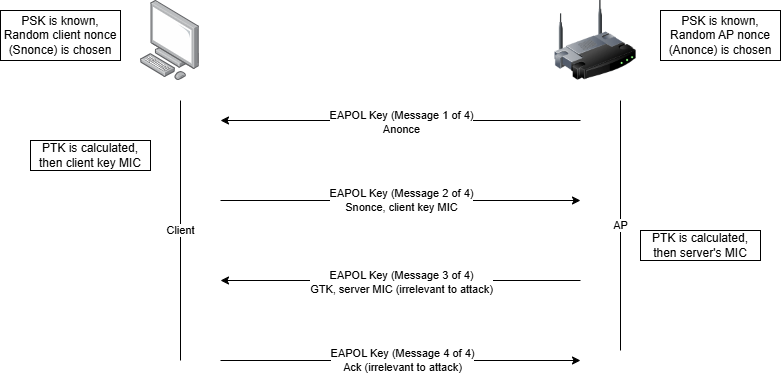
\includegraphics[width=0.45\textwidth]{four_way_handshake.png}
    \caption{The four way handshake: focusing on information relevant to our attack}
\end{figure}

After both the client and AP possess the PMK and nonces, the four way handshake begins: four EAPOL (Extensible Authentication Protocol over LAN) packets, sent between the AP and client, that should prove that the client possesses the correct PSK, by proving they possess the correct PMK (and relying on the collision resistance of the hashing algorithm).

The first handshake packet is sent from the AP to the client; in it, the server nonce, or ANonce, is sent. After receiving the first packet, the client derives the PTK (Pair Temporary Key) by PRF (pseudo-random function). Two salts are used for the PTK calculations; one is constant, and is the string "Pairwise key expansion", called the "A" salt, and the second is dynamic, calculated from the client and AP MAC addresses, along with the two nonces, called the "B" salt.
The PTK is then split into three different keys: the Key Confirmation Key (KCK), Key Encryption Key (KEK)
and Tempotal Key (TK); only the KCK is relevant to our attack, and 
is then used to produce the client key MIC (Message Integrity Code) \cite{alhamry2022exploring}, \cite{abo2017study}, \cite{arana2006benefits}. 

The client sends the second packet to the AP, containing their nonce (SNonce) and the client key MIC. At this point, it's critical to understand that given a passphrase guess, all information needed to calculate the client key MIC ourselves is present in the first two four way handshake packets, as long as we know the SSID in addition, which can be found in a beacon packet sent before. This means that given these three packets only, a network adversary can perform a dictionary or brute force attack, calculating the client key MIC and comparing it to the one sent in the second handshake packet. For this reason, the last two packets in the handshake are irrelevant to us, and will not be discussed further.

The exact calculation performed is:
\begin{enumerate}
\item  PMK is derived by sha1-hmac based PBKDF2, on the PSK, ssid, ssidLength, iterations constant (4096) and length constant (256).
\item  The B salt is calculated from the MAC addresses and nonces, by min(AP\_MAC, S\_MAC) || max(AP\_MAC, S\_MAC) || 

min(APNonce,SNonce) || max(APNonce,SNonce)
\item The PTK is derived by HMAC-based (Hash Based Message authentication Code) PRF on the PMK, A salt ("Pairwise key expansion") and B salt.
\item The client key MIC is calculated by custom HMAC from the PTK, the EAPOL Authentication layer of the second handshake packet, with the MIC zeroed out (as it hasn't been calculated yet).
\end{enumerate}

The current state-of-the-art for cracking passwords is johntheripper \cite{john}.

\subsection{Attack Description}

We've created a Python library called `eyalthesinger`, with the hope of making it installable via `pip`, in which our attack is implemented. We also implemented different versions of the attack in the CTF challenges, which are discussed in the next section.

Our library provides a CLI and is in fact runnable. This CLI is the entrypoint to our attack, and also provides high-level which are easier and we thought \textit{should} be implemented in Python like downloading a wordlist (example: `eyalthesinger download rockyou`), handling a server and clients (example: `eyalthesinger server` and `eyalthesinger connect`), and later on a `format` subcommand which enables to parse a PCAP and format it as something that can be easily brute-forced.

We created a WPA format tool that receives a .pcap file containing a sniffed connection to a wifi network, filters for the first two of the four way handshake packet, and for the additional beacon packet (for the SSID, as described in the previous section) in order to be able to use the necessary information quickly by a C program. It is delimited by colons and includes (in this order):
\begin{itemize}
\item null-terminated SSID (e.g. `b"TAU-Free"`).
\item the client MAC (SMac).
\item the AP MAC (APMac).
\item The client nonce (SNonce).
\item The server nonce (ANonce).
\item The second packet's EAPOL layer bytes (used for the MIC calculation as discussed before; without the MIC zeroed out).
\item The client key MIC.
\end{itemize}

We implemented our own cryptography for the attack, as we wanted to improve our cracking speed by implementing the cryptographic functions on our own. This is because as we know OpenSSL implements \textit{security measures} for coping with side channel attacks, and when we're brute-forcing a password we don't want to pay the \textit{performance hit} incurred by this. The function we implemented are: sha256, sha1, hmac-sha1, hmac-sha1 based pbkdf2. All functions are implemented in C.

For the actual "meat" of the library, there is the `crack` command. We offer both WPA2 cracking, and sha256 cracking. This command calls a C program named `sing` which is intended to be \textit{very} fast, and from our experimentation beats the speed of `johntheripper` (using OpenSSL), at least for sha256 cracking \footnote{\hyperlink{https://github.com/openwall/john}{https://github.com/openwall/john}}.

Our WPA2 cracker calculated the client key MIC by:
\begin{enumerate}
\item  Calculating the PMK by sha1-hmac based PBKDF2, which we implemented ourselves, on the PSK, ssid, ssidLength, iterations constant (4096) and length constant (256).
\item  Calculating from the MAC addresses and nonces, by min(AP\_MAC, S\_MAC) || max(AP\_MAC, S\_MAC) || min(APNonce,SNonce) || max(APNonce,SNonce)
\item Calculating the PTK is by our own implementation of HMAC-based (Hash Based Message authentication Code) PRF-512 on the PMK, A salt ("Pairwise key expansion") and B\_salt. In the algorithm, PRF-383 is used; however, PRF-512 was easier to implement, and the first 383 bits are the same. As we only use the KCK (see previous section) anyway, which is only the first 128 bits, this doesn't matter.
\item Calculating the client key MIC by custom HMAC from the KCK, the EAPOL Authentication layer of the second handshake packet, zeroing out the MIC.
\end{enumerate}

Our tool goes over the specified wordlist, calculates the client key MIC for each password, and compares it to the client key MIC from the second handshake packet. The `crack` command automatically uses multi-processing (in python), splitting the wordlist according to the number of GPU's available.

We've also tried to enable GPU parallelization for the library, and eventually succeeded in using CUDA to break SHA256; However, as it was too slow for WPA2 and the interface it posed was challenging, we decided to focus on networking instead.

Finally, we implemented network parallelization: the `server` and `connect` functions. The REPL server has supports the `download` and `crack` commands from our library; It listens for incoming connections, and asks for CPU information from each client upon connecting. The clients (used by `connect`) automatically send that information and wait for further instructions. Upon receiving a `crack` instruction from the user, the server splits the wordlist specified between all connected clients, taking the CPU's available for each client into account. It then waits for one of the clients to succeed.

\subsection{Design}

We aimed to create a CTF challenge that familiarizes the user with the attack on the WPA2 protocol, step by step, while also learning about dictionary and brute force attacks, and the benefits of multi-threading. We also wanted to emphasize the importance of a strong password. We chose to use the CTFd \footnote{\hyperlink{https://github.com/CTFd/CTFd}{https://github.com/CTFd/CTFd}} platform, as we have used it before, and found it extremely user-friendly. 

Our CTF has 4 main sections:
\begin{enumerate}
\item Introduction- the players get a “free” flag at the beginning, after reading about the goals of the CTF, and after reading a legal disclaimer about misusing the methods that appear in the CTF.
\item SHA-256 challenges- these challenges serve as a “warmup”, by getting the users familiar with the brute force process, and have them use multithreading, before learning about WPA2.
\item WPA2 challenges- these challenges aim to get the user familiar with the WPA2 protocol, the 4-way handshake, and the offline attack. This is the main part of the CTF.
\item Fast WPA2- the final challenge that combines all the previous ones, and tests the players’ efficiency. We created a server that sends them WPA2 dictionary attack challenges, and requires them to utilize multithreading in order to get the flag.
\end{enumerate}

For each challenge, we created a pdf file containing all of the necessary instructions and information, and for some challenges, we also provide the players a basic outline of the code.

We chose to address players with different backgrounds in two ways: First, we created additional materials that can be given to players who aren't familiar with different technological concepts, that include explanations necessary for completing the CTF successfully, along with links for further reading on each topic. The materials include:
\begin{itemize}
\item Hashing and sha256.
\item Brute force and dictionary attacks.
\item Multithreading.
\item Networking and wireshark.
\end{itemize}
In addition, in the WPA2 category challenges, we provide the players with a .pcap file containing a four way handshake and additional beacon packet (needed for the SSID) in each challenge. For beginner players, we provide a .pcap file containing only these five packets, so they can focus on understanding how to handle packets in wireshark; for experienced players, we provide a .pcap file with more traffic for some of the challenges, so that they will need to filter for the packets.

\subsubsection{Introduction}

The first “challenge” consists only of a PDF file; in it the players learn about the goals of the CTF activity. We also included a version of the disclaimer sent to us at the beginning of the course, explaining the dangers of using the methods shown in the CTF, and warning them about the legality. After reading the file, they receive a “free” flag.

\subsubsection{SHA-256 challenges}
In these challenges, we “warm up” the players, get them to write some code, and get them familiarized with brute-force and multithreading.

\begin{enumerate}
\item Dictionary attack:
  In the first challenge, the players receive the RockYou \footnote{\hyperlink{https://github.com/brannondorsey/naive-hashcat/releases/download/data/rockyou.txt}{https://github.com/brannondorsey/naive-hashcat/releases/download/data/rockyou.txt}} leaked password list, and the sha-256 hash of one of the passwords. They are asked to perform a dictionary attack in order to discover the password.  
  They also receive our implementation of sha-256, and a simple shell of the code (both written in c) needed to perform the dictionary attack. Since we implemented our own version of sha-256 (as described in the previous sections), there is no use of external libraries, other than standard (stdio, stdint, string), in this challenge. 
  The flag in this challenge is the password.
  
\item Brute force using multithreading:
  In the second challenge, the players should already be familiar with sha-256 and dictionary attacks, and so we up the difficulty: this time, the players receive the hash of a password of unknown length, chosen from a specific charset, and are asked to use brute-force to discover the password.
  We chose a password of length 5, that, by our estimations, should take almost an hour to reach by brute force without using multithreading. So, the users must learn to utilize multithreading in order to successfully pass this challenge in a feasible timeline.
  As before, the players receive our implementation of sha-256, and a simple shell of the code. Only multithreading and standard libraries are needed for this challenge.
  The flag in this challenge is the password.
\end{enumerate}

\subsubsection{WPA2 challenges}
After the players are familiar with dictionary attacks, brute force and multithreading, we introduce them to the WPA2 protocol. As the protocol is a bit difficult, we created multiple challenges, exposing the players to the concepts little by little.

\begin{enumerate}
\item Understanding the four way handshake:
  The first challenge’s aim is mainly to get the players familiar with the protocol itself, without needing to implement anything. We provide them with background materials that include detailed explanations of the protocol, that should be read and understood before proceeding.
  In addition, we provide them with a .pcap file the four way handshake packets, and the additional beacon packet needed for the SSID (as this is the first challenge, we only provide these 5 packets). They are asked to find the client key MIC in the packets, and enter it as the flag.
\item Calculating the client key MIC:
  In this challenge, we provide the players with the four-way handshake packets and the beacon packet, this time with the client key MIC removed from the second handshake packet. We also provide them with the password used for this connection.
  We ask them to calculate the client key MIC from the password and the other fields included in the .pcap file, and enter it as the flag.
  We provide the players with a shell of the code that performs this calculation in c, and with a detailed explanation of the protocol and calculations performed.
  As this is, in our opinion, the most difficult challenge, as it requires a full understanding of the protocol, the shell is the most detailed here: we provide detailed documentation of all the functions that they need to implement, as well as declarations of all the constants they need to find and use. There will also be more hints offered in this challenge (described in the next section).
  As we implemented our own cryptography for the calculations needed (as described in the previous sections), only standard libraries need to be used for this challenge.
\item Dictionary attack:
  After successfully calculating a client key MIC, the players are now ready to perform a dictionary attack.
  They are provided with a partial RockYou file, containing 5000 passwords, and a .pcap file containing the four way handshake packets and beacon packet, of a connection that used some RockYou password from the partial list. For this challenge and the next one, we start providing the "experienced" option for the .pcap captures.
  The players are asked to perform a dictionary attack and discover the password, then enter it as the flag.
  As this challenge heavily relies on their code from the previous challenge, they are not provided with any more code.
\item Brute force attack:
  Similarly, the players are provided here with a .pcap file containing the four way handshake packets and beacon packet, and a trivia fact that many people in Israel use phone numbers as wifi passwords. They are asked to perform a brute force attack. As brute forcing the entire phone number takes too long, they are also given the beginning of the number, leaving 4 digits unknown. As before, they are not provided with any extra code, and the flag is the password itself.
\item Bonus challenge:
  We added one special challenge to this section, in which the players are asked to sniff a connection themselves, and filter out the four way handshake packets by themselves. We thought that including this challenge as part of the the previous challenges in this section, might take the emphasis off of their main goal, so we added it as a bonus. We do still believe that sniffing and filtering for the packets can give the players a nice introduction to networking, packets and .pcap files.
  In this challenge, the players are asked to show us (or to whoever is running the CTF) that they are able to sniff and filter the packets. If successful, they will be told the flag.
  \end{enumerate}

\subsubsection{Fast WPA2}
In the final section of the CTF, the players are asked to combine everything that they learned so far. They receive a server file (as an executable), and a partial client file.
The server chooses a random RockYou password from a partial file containing 100,000 passwords, and calculates the MICs of 100 passwords (“1” to “100”) in order to estimate how long it will take this device to go over the entirety of the list. It then sends the information from a theoretical connection that uses the chosen random password (client key MIC, ssid and all other relevant information for the .pcap files in the previous challenges) to the client, with a time limit of 1/8th of the time it would take to go through the entirety of the list. If the client manages to perform the dictionary attack and send the password back to the server in time, they receive the flag. Otherwise, they need to try again.
This forces the players to use multithreading in order to answer the challenge in time.
We thought this challenge serves both as a nice conclusion to the CTF, and teaches the players how fast it actually is to perform a dictionary attack, even with one "regular" computer only.
We would also like to mention that we encrypted the flag so that a simple “strings” command won’t reveal it.


\subsection{CTF Instructions}

In order to run the CTF, a good understanding of the WPA2 protocol is needed (in order to be able to assist the players). We suggest reading the background material provided in the first WPA2 challenge (can be found under ctf/4\_wpa2\_1/wpa2\_explanation.pdf).
We organized the materials needed for each challenge in its own directory,with each challenge containing:
\begin{itemize}
\item A zip file, containing all files needed for each challenge. Under the WPA2 category, there is also a second zip file for some of the challenges, ending with "experienced", for experienced players, as described in the previous section.
\item a “solutions” sub-directory- we also recommend looking at the implementations we provided before running the CTF. Under “solutions”, there is also a “hints.txt” file containing every clue we think should be given; In our CTFd server, we included them already, as “paid hints”, meaning the players lose a certain amount of points in order to reveal a clue.
\end{itemize}

The challenges currently uploaded to the server are the beginner level versions of the WPA2 challenges,but we encourage anyone running the ctf to switch the files accordingly.
In addition, the additional materials for beginner players described in the previous challenges are present under "ctf/additional\_materials". The files should be provided to anyone in need of assistance; they are also currently uploaded to the ctf server.

The CTF is hosted on \hyperlink{https://server.noamzaks.com}{https://server.noamzaks.com}.
Using the site is pretty straightforward- we uploaded all of the challenges and necessary materials. The players should download the files for each challenge, start by reading the detailed instructions we provided (as a pdf file, inside each challenge's zip file), and then start implementing their code. They can "pay" for hints, also uploaded to the site, and at the end need to enter the flag.


\subsection{Conclusion}

In this project, we explored and exploited vulnerabilities in the WPA2 security protocol by developing a tool that performs offline dictionary and brute-force attacks on a Wi-Fi connection, discovering the Wi-Fi's passphrase. We showed how weak password choices can lead to serious security risks, and how important it is to choose a good password.

We also designed a CTF challenge that provides participants with a hands-on learning experience. The challenge guides the participants through building a very powerful tool of their own, that allows them to see how predictable passwords can be exploited. We hope to encourage a better understanding of Wi-Fi security, and to continue inspiring technological curiosity. We try to emphasize security awareness throughout the challenges, and hope we can instill them in the participants.

This project serves as a reminder that even widely used and trusty security protocols like WPA2 are only as strong as their weakest link, the passwords chosen by their users.

\subsection{Contributions}

We started the project with researching the attack together as a group, and implementing the base WPA2 cracker (client key MIC calculation) together. After that, we started splitting the work between us.

\begin{itemize}
\item Maya Ben Shalom:
    \begin{itemize}
  \item Network parallelization implementation.
  \item Dictionary and brute force attacks on WPA2 (joint with Eliav Huppert).
  \item CTF design, focusing on the introduction and WPA2 category challenges, including the WPA2 category solutions.
  \item CTFd server design.
  \end{itemize}
  
\item Gal Chapman:
\begin{itemize}
  \item Protocol research.
  \item Cryptographic implementations.
  \item Sniffing connections and formatting them for WPA2 cracking.
  \item Script that creates all of the .pcap captures for the CTF's WPA2 category challenges.
\end{itemize}
  
\item Eliav Huppert:
    \begin{itemize}
  \item GPU parallelization.
  \item Dictionary and brute force attacks on WPA2 (joint with Maya Ben Shalom).
  \item CTF design, focusing on the sha256 and fast WPA2 category challenges, including all solutions.
  \end{itemize}
  
\item Noam Zaks:
\begin{itemize}
  \item Infrastructure (base C and Python layout).
  \item Download command and WPA2 multiprocessing in python.
  \item Base SHA256 cracker.
  \item CTFd server creation.
  \end{itemize}
\end{itemize}

At the end of the individual work, we came together again to write this report, each of us contributing, and to plan the final presentation of our project.






%%
%% The acknowledgments section is defined using the "acks" environment
%% (and NOT an unnumbered section). This ensures the proper
%% identification of the section in the article metadata, and the
%% consistent spelling of the heading.
% \begin{acks}
% Acknowledgements go here. Delete enclosing begin/end markers if there are no acknowledgements.
% \end{acks}

%%
%% The next two lines define the bibliography style to be used, and
%% the bibliography file.

\bibliographystyle{ACM-Reference-Format}
\bibliography{refs.bib}

%%
\end{document}
\endinput
%%
%% End of file `main.tex'.
